% !TeX encoding=utf8
% !TeX spellcheck = de-DE

\section{Produktdaten}
\newcolumntype{s}{>{\hsize=.15\hsize}X}


\begin{tabularx}{\linewidth}{s X}
	\texttt{/D010/} & \textbf{Benutzerdaten}: Alle Daten die über einen Benutzer des Systems gespeichert werden.
	\begin{itemize}
		\item BenutzerID (eindeutig)
		\item Rolle (Entwickler, Projektleiter oder Teamleiter)
		\item Kennung \begin{itemize}
			\item Benutzername (eindeutig)
			\item Kennwort (verschlüsselt)
		\end{itemize}
		\item Name
		\item E-Mail Adresse
		\item Zugehörigkeit zu Teams (können mehrere sein)
	\end{itemize}
	\\
	 \texttt{/D020/} & \textbf{Teamdaten}: Alle Daten die die einzelnen Teams und ihre Zusammensetzung betreffen.
	 \begin{itemize}
	 	\item TeamID (eindeutig)
	 	\item Eine Liste der Teams
	 	\item Mitglieder der Teams und welchen Teams sie angehören.
	 	\item Teamleiter
	 	\item Den Teams zugeordnete Tasks
	 \end{itemize}
 	\\
 	 \texttt{/D030/} & \textbf{Projektdaten}: Alle Daten bezüglich laufender Projekte.
 	 \begin{itemize}
 	 	\item ProjektID (eindeutig)
 	 	\item Projektname
 	 	\item Dem Projekt zugewiesene Teams
 	 	\item Eine Beschreibung des Projekts
 	 	\item Das Ausgewählte Vorgehensmodell des Projekts. (Keins, Wasserfall, V-Modell, Spiralmodell)
 	 	\item Die Projektphasen entsprechend dem Vorgehensmodell \begin{itemize}
 	 		\item Aktuelle, nächsten und vorhergehenden Phasen
 	 	\end{itemize}
 	 \end{itemize}
	\\
\end{tabularx}
\clearpage
\begin{tabularx}{\linewidth}{s X}
	\texttt{/D040/} & \textbf{Task - Daten}: Alle Daten über Tasks welche in Bearbeitung, beendet oder geplant sind.
	\begin{itemize}
		\item TaskID (eindeutig)
		\item Deadline für die Task
		\item Zeitstempel an dem die Task abgeschlossen wurde
		\item Name und Beschreibung des Tasks
		\item Zugeteilte Projektphase(n)
		\item Abhängigkeiten und Reihenfolgen zu anderen Tasks
		\item Task Label
		\item Kommentare der Entwickler
	\end{itemize}
\end{tabularx}
\subsection{Datenbankschema}
\begin{figure*}[h!]
	\centering
	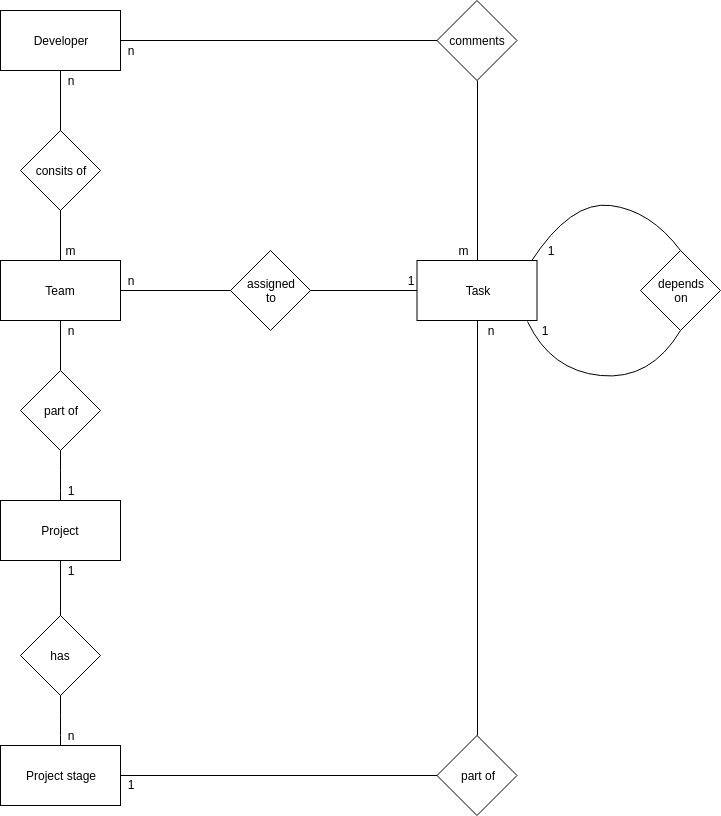
\includegraphics[width=0.65\textwidth]{owlkeeper_database.png}
\end{figure*}

